\section{Diskussion}
Bei Betrachtung der Ergebnisse für den Fluss in Abbildung \ref{fig:Fluss} fällt auf, dass die beiden Entfaltungsmöglichkeiten zu einem nahezu identischen Ergebnis führen. Die Punkte liegen in den meisten Fällen übereinander, lediglich für hohe Energien ergeben sich Abweichungen.

Für die Unsicherheiten der Likelihood-Entfaltung, fällt auf, dass besonders bei hohen Energien der Fluss hohe Unsicherheiten besitzt. Dieses liegt daran, dass in diesem Energiebereich deutlich weniger Ereignisse zu finden sind. Dadurch wird der statistische Fehler auf die Größen erhöht. Die erhöhten Unsicherheiten auf die hohen Energiewerte können möglicherweise zu den Abweichungen der Entfaltungsmethoden in diesem Bereich führen.

\begin{figure}
	\begin{subfigure}[c]{0.5\textwidth}
		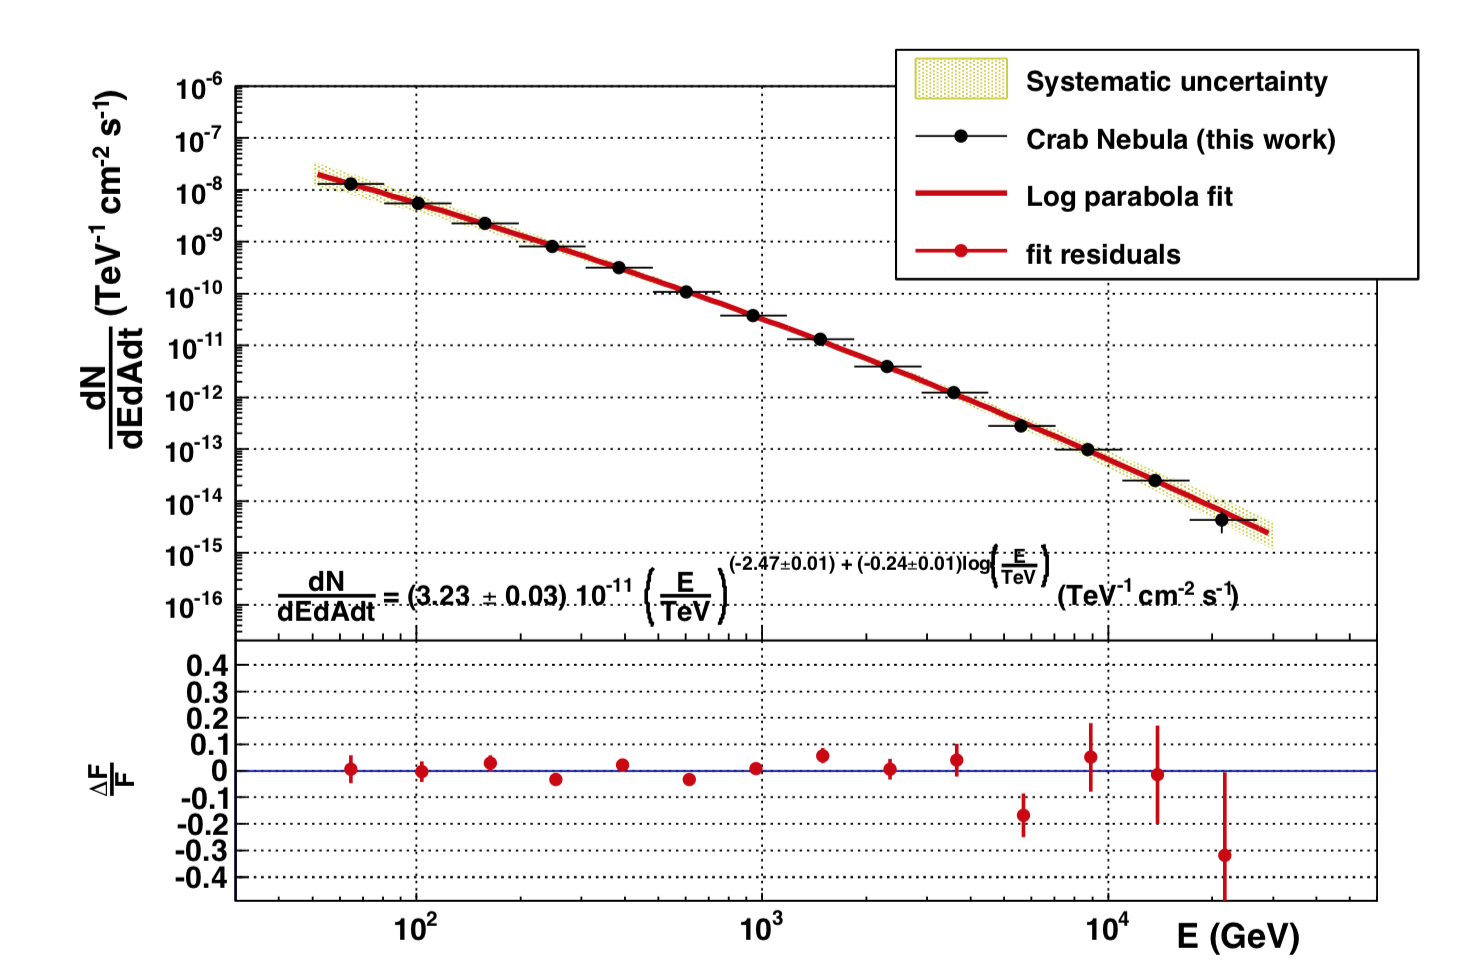
\includegraphics[width=\textwidth]{graphics/Magic.png}
		\subcaption{Der von der MAGIC Kolloboration bestimmte Fluss des Krebsnebels.\cite{Aleksic:2014jva}}
	\end{subfigure}
	\begin{subfigure}[c]{0.5\textwidth}
		\includegraphics[width=\textwidth]{plots/Fluss_Like.pdf}
		\subcaption{Der mit Likelihood-Entfaltung bestimmte Fluss des Krebsnebels.}
	\end{subfigure}
	\caption{Vergleich der Messungen zum Fluss des Krebsnebels mit MAGIC und FACT Daten.}
\end{figure}
\FloatBarrier
Im Vergleich der berechneten Flusswerte des Krebsnebels aus der Entfaltung der FACT-Daten mit denen aus der Veröffentlichung \cite{Aleksic:2014jva} der MAGIC Kolloboration fällt auf, dass der Fluss nahezu in der selben größen Ordnung liegt. Der Fluss aus den FACT-Daten ist lediglich ein wenig geringer. Die Abweichungen können mit den unterschiedlichen Detektorsystemen begründet werden. Beide Daten folgen demselben abfallenden Trend. Somit kann an dieser Stelle von einer gelungenden Entfaltung der Messdaten und einer sinnvollen Flussberechnung ausgegangen werden.
